\section{Introduction}
\label{sec:intro}

Robot-assisted surgery produces hours of endoscopic video, and the automatic analysis of that video underpins workflow analysis, skill assessment, context-aware assistance and, further out, partial automation of surgical steps \citep{ayobi2024pixel}.
All of these need the same visual foundation: which instruments are in the field of view, where they are, and which kind each one is.
Instrument recognition, the segmentation of every instrument together with its type, is therefore a basic building block of surgical scene understanding \citep{gonzalez2020isinet,ayobi2023matis}.

Naming the type of an instrument is harder than segmenting ``a tool''.
Instruments of different types share shafts, wrists and jaws, and the parts that tell them apart are often out of frame, occluded, or turned away from the camera.
Figure~\ref{fig:teaser} shows a typical case from the GraSP benchmark.
A Laparoscopic Grasper enters the keyframe at the edge of the view, and a classifier that sees only this frame believes it is a Prograsp Forceps (belief 0.57) and is visibly unsure.
A few seconds earlier or later the same instrument is seen from a clearer angle and is classified correctly, and combining the frames recovers the right class.
Temporal context is thus the natural remedy for ambiguous views, but it is not free: it requires following each instrument through the video and classifying it again on every frame, and most instruments do not need it.
The practical question is not whether to use temporal context but where.

\begin{figure}[t]
\floatconts
  {fig:teaser}
  {\caption{A single frame can be ambiguous, neighbouring frames are not. (a)~The keyframe with the box that is given and the mask a segmenter predicts for it. (b)~The class belief of the evidential ensemble from the keyframe alone (grey) and fused over the frames in (c) (teal); the true class is in green. (c)~Neighbouring frames with the propagated mask; the label under each is the prediction from that frame alone. The keyframe prediction is wrong and uncertain, so the instrument is sent to temporal correction, which fixes it. Most instruments are not uncertain and never need it.}}
  {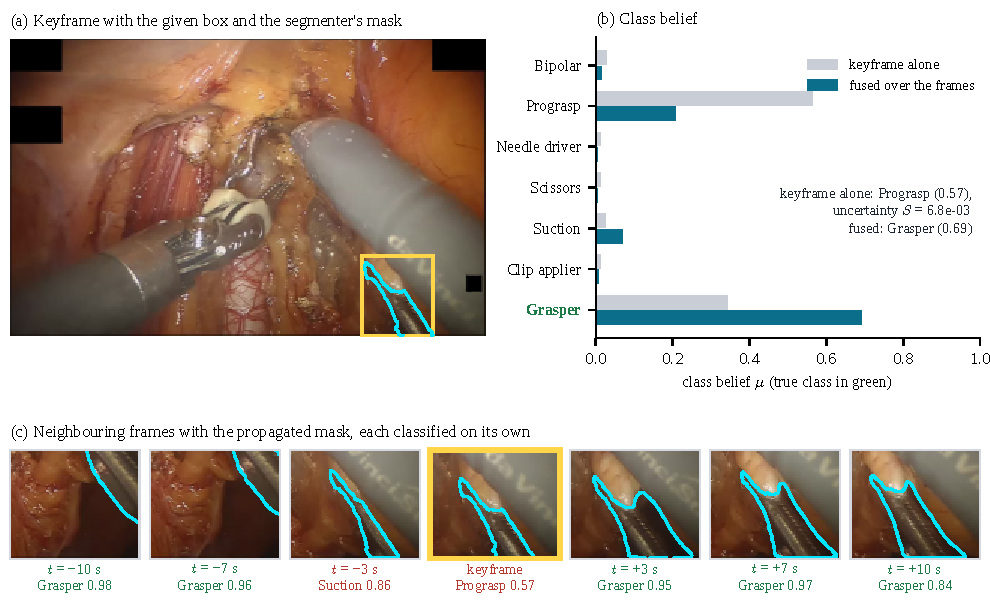
\includegraphics[width=\linewidth]{figures/fig1_example.pdf}}
\end{figure}

The strongest published system on this benchmark, TAPIS \citep{ayobi2024pixel}, detects and classifies instruments with a Mask2Former detector \citep{cheng2022mask2former} and adds a video transformer that reads a clip of frames around every keyframe.
It spends the same temporal budget on every instrument and does not use an uncertainty estimate to decide where that budget is needed.
Annotated surgical frames are also few and the classes are imbalanced, the rarest instrument having about 25 times fewer examples than the most common, which favours models that start from strong pretrained representations.
Promptable segmentation models now provide those representations for masks: given a box, SAM2 and SAM3 return a mask \citep{ravi2024sam2,carion2025sam3}, but neither says what the object is.

We therefore separate \emph{where} from \emph{what}, and spend temporal context only where it is needed.
A given box prompts fine-tuned SAM2 and SAM3 segmenters; a light four-member evidential ensemble classifies the masked crop in a single pass and returns, besides the class, an epistemic uncertainty \citep{sensoy2018evidential,duan2024evidential}; only instruments whose uncertainty passes a gate are followed by SAM2 through neighbouring frames, and the per-frame predictions are fused by confidence (Section~\ref{sec:method}).
We assume the boxes are given.
Surgical instrument detectors are already strong (TAPIS reports 89.85 box mAP at an IoU of 0.5 on this data), so we study recognition given boxes and leave the integration of a detector to future work (Section~\ref{sec:limits}).

On GraSP this reaches 87.4 mIoU, 86.2 IoU and 78.3 mcIoU against 86.6, 83.4 and 77.4 for TAPIS, which finds its own boxes (Section~\ref{sec:results}).
The evidential score detects errors as well as MC dropout with one forward pass instead of eighty and, unlike a vote, flags errors on which all members agree (Section~\ref{sec:uncertainty}).
A causal variant for streaming video, with a small segmenter and a causal tracker, keeps most of the accuracy (Section~\ref{sec:realtime}).
Our contributions are:
\begin{itemize}
\item an evidence-gated pipeline that decides in one forward pass which instruments receive temporal correction, with a tracker-style-crop training scheme that prepares the classifier for the crops a tracker produces;
\item a comparison of evidential and MC-dropout uncertainty as the gate signal, at equal or better error detection and one eightieth of the cost;
\item a causal, one-frame-per-second variant with accuracy and latency reported together.
\end{itemize}
